\section{Program \texttt{lalapps\_inspinj}}
\label{program:lalapps-inspinj}
\idx[Program]{lalapps\_inspinj}

\begin{entry}
\item[Name]
\verb$lalapps_inspinj$ --- produces inspiral injection data files.

\item[Synopsis]
\verb$lalapps_inspinj$ \newline
%
[\texttt{--help}]\newline
\texttt{--source-file} \textsc{sfile} \newline
\texttt{--mass-file} \textsc{mfile}\newline
%
[\texttt{--gps-start-time} \textsc{tstart}]\newline 
[\texttt{--gps-end-time} \textsc{tend}]\newline
%
[\texttt{--time-step} \textsc{tstep}] \newline
[\texttt{--time-interval} \textsc{tinterval}]\newline
%
[\texttt{--seed} \textsc{seed}]\newline
[\texttt{--waveform} \textsc{wave}]\newline
[\texttt{--lal-eff-dist}]\newline
[\texttt{--usertag} \textsc{tag}]\newline
%
[\texttt{--tama-output}]\newline
[\texttt{--write-eff-dist}]\newline
%
[\texttt{--ilwd}]

\item[Description] 
\verb$lalapps_inspinj$
generates a number of inspiral  parameters suitable  for using in a Monte
Carlo injection to test the efficiency of a inspiral search.  The  various
parameters (detailed  below)  are randomly chosen and are appropriate for a
particular population of binary neutron stars  whose spatial  distribution
includes the Milky Way and a number of extragalactic objects that are  input
in  a  datafile.  The  possible  mass pairs for the binary neutron star com-
panions are also specified in a (different) datafile.

The output of this program  is  a  list  of  the  injected events,  starting
at  the specified start time and ending at the specified end time.  One 
injection with random inspiral parameters will be made every specified time
step, and will be randomly placed within the specified time interval.  
The output is written to a file name in the standard inspiral pipeline format:
\begin{center}
\begin{verbatim}
HL-INJECTIONS_USERTAG_SEED-GPSSTART-DURATION.xml
\end{verbatim}
\end{center}
where \verb$USERTAG$ is \textsc{tag} as specfied on the command line, 
\verb$SEED$ is the  value  of  the random number seed chosen and 
\verb$GPSSTART$ and \verb$DURATION$ describes the GPS time interval that
the file covers. The file is in the standard LIGO lightweight XML format
containing a \texttt{sim\_inspiral} table that describes the injections.
In addition, an ASCII log file called \verb$injlog.txt$ is also written.
If a \texttt{--user-tag} is not specified on the command line, the
\texttt{\_USERTAG} part of the filename will be omitted.

\item[Options]\leavevmode
\begin{entry}
\item[\texttt{--help}] Print a help message.

\item[\texttt{--source-file} \textsc{sfile}]
Optional. Data file containing spatial distribution of  extragalactic  objects.
Default  is  the file \verb+inspsrcs.dat+ provided by LALApps. If that file is 
empty, all signals are in the Milky Way.

\item[\texttt{--mass-file} \textsc{mfile}]
Optional. Data file containing mass pairs  for  the binary  neutron  star
companions.   Default is the file \verb+BNSMasses.dat+ provided by LALApps.

\item[\texttt{--gps-start-time} \textsc{tstart}]
Optional.  Start time of the injection data to be created. Defaults to the
start of S2, Feb 14 2003 16:00:00 UTC (GPS time 729273613)

\item[\texttt{--gps-end-time} \textsc{tend}]
Optional. End time of the injection data to be created. Defaults to the end of
S2, Apr 14 2003 15:00:00 UTC (GPS time 734367613).

\item[\texttt{--time-step} \textsc{tstep}]
Optional. Sets the time step interval between injections. The injections will
occur with an average spacing of \textsc{tstep} seconds. Defaults to 
$2630/\pi$.

\item[\texttt{--time-interval} \textsc{tinterval}]
Optional. Sets the time interval during which an injection can occur. 
Injections are uniformly distributed over the interval.  Setting \textsc{tstep}
to $6370$ and \textsc{tinterval} to 600 guarantees there will be one injection
into each playground segment and they will be randomly distributed within the
playground times - taken the fact that your gps start time coincides with start of a playground segment.

\item[\texttt{--seed} \textsc{seed}]
Optional. Seed the random number generator with the integer \textsc{seed}.
Defaults to $1$.

\item[\texttt{--waveform} \textsc{wave}]
Optional. The string \textsc{wave} will be written into the \texttt{waveform}
column of the \texttt{sim\_inspiral} table output. This is used by the
inspiral code to determine which type of waveforms it should inject into the
data. Defaults is \texttt{GeneratePPNtwoPN}.

\item[\texttt{--lal-eff-dist}]
Optional.  If this option is specified, the effective distance will be
calculated using routines from LAL.  Otherwise, the default behaviour is to
use an independent method contained in inspinj.c.  There is good agreement
between these two methods, see below for more details.

\item[\texttt{--user-tag} \textsc{string}] Optional. Set the user tag for this
job to be \textsc{string}. May also be specified on the command line as 
\texttt{-userTag} for LIGO database compatibility.

\item[\texttt{--tama-output}]
Optional.  If this option is given, \verb+lalapps_inspinj+ also produces a 
text output file:
\begin{center}
\begin{verbatim}
HLT-INJECTIONS_USERTAG_SEED-GPSSTART-DURATION.txt
\end{verbatim}
\end{center}
which contains the following fields:

\begin{itemize}
\item geocentric end time
\item Hanford end time
\item Livingston end time
\item TAMA end time
\item total mass, $M_{\mathrm{TOT}}$
\item mass ratio, $\eta$
\item distance to source (in kpc)
\item longitude
\item latitude
\item inclination
\item coalescence phase
\item polarization
\item TAMA polarization
\item end time GMST
\end{itemize}

In the above, all times are recorded as double precision real numbers and all
angles are in radians.  The TAMA polarization is calculated using
%
\begin{equation}
  \tan( \psi_{T} ) = \frac{ x \cdot T_{z} }{ y \cdot T_{z} } \, .
\end{equation}
%

Here x and y are the x,y axes of the radiation frame expressed in earth fixed
coordinates (\ref{xrad}, \ref{yrad}).  $T_{z}$ is a unit vector in earth fixed
coordinates which is orthogonal to the two arms of the TAMA detector
(\ref{tarm}).  It is given by

%
\begin{equation}
  T_{z} = ( -0.6180, +0.5272, +0.5832 )
\end{equation}
%

\item[\texttt{--write-eff-dist}] Optional.  If this option is given, three extra
columns are added to the TAMA output file described above.  They are
\begin{itemize}
\item Hanford effective distance (kpc)
\item Livingston effective distance (kpc)
\item TAMA effective distance (kpc)
\end{itemize}
  
These entries are added to the list immediately after TAMA end time and before
total mass.

\item[\texttt{--ilwd}] Optional. If this option is given,
\verb+lalapps_inspinj+ also produces two ILWD-format files, injepochs.ilwd and
injparams.ilwd, that contain, respectively, the  GPS  times  suitable for
inspiral injections, and the intrinsic inspiral signal parameters to be used
for  those injections.

The  file  injepochs.ilwd  contains  a sequence of integer pairs representing
the injection GPS time in  seconds  and residual  nano-seconds.   The file
injparams.ilwd contains the intrinsic binary parameters for each injection,
which is  a  sequence  of  eight  real  numbers representing (in order) (1) the
total mass of the binary system  (in  solar masses),  (2)  the  dimensionless
reduced mass --- reduced mass per unit total mass --- in the range from  0
(extreme mass  ratio)  to  0.25 (equal masses), (3) the distance to the system
in meters, (4) the inclination  of  the  binary system  orbit  to the plane of
the sky in radians, (5) the coalescence phase in radians, (6)  the  longitude
to  the direction  of  the  source in radians, (7) the latitude to the
direction of the source in radians, (8) and the polar- ization angle of the
source in radians.
\end{entry}

\item[Example]
\begin{verbatim}
lalapps_inspinj --seed 45\
--source-file inspsrcs.dat --mass-file BNSMasses.dat
\end{verbatim}


\item[Algorithm]

The algorithm for computing the effective distance will be described in some
detail below.  The method is to compute both the strain due to the inspiral
and the detector response in the earth fixed frame.  This frame is such that
the z-axis points from the earth's centre to the North Pole, the x-axis points
from the centre to the intersection of the equator and the prime meridian and
the y-axis is chosen to complete the orthonormal basis.  The coordinates of
the injection are specified by longitude (or right ascension) $\alpha$ and
latitude (or declination) $\delta$.  The polarization is appropriate for
transferring from the radiation to earth fixed frame.  These are then
converted to the earth fixed frame by
%
\begin{eqnarray}
  \theta &=& \frac{\pi}{2} - \delta \\
  \phi &=& \alpha - \textrm{gmst} \, .
\end{eqnarray}
%
Here, gmst is the Greenwich Mean sidereal time of the injection.  The axes of
the radiation frame (x,y,z) can be expressed in terms of the earth fixed
coordinates as:
%
\begin{eqnarray}
  x(1) &=& +( \sin( \phi ) \cos( \psi ) - \sin( \psi ) \cos( \phi ) 
      \cos( \theta ) ) \nonumber \\
  x(2) &=& -( \cos( \phi ) \cos( \psi ) + \sin( \psi ) \sin( \phi ) 
      \cos( \theta ) ) \nonumber \\
  x(3) &=& \sin( \psi ) \sin( \theta ) \label{xrad}\\
  y(1) &=& -( \sin( \phi ) \sin( \psi ) + \cos( \psi ) \cos( \phi ) 
      \cos( \theta ) ) \nonumber\\
  y(2) &=& +( \cos( \phi ) \sin( \psi ) - \cos( \psi ) \sin( \phi ) 
      \cos( \theta ) ) \nonumber \\
  y(3) &=& \cos( \psi ) \sin( \theta ) \label{yrad}
\end{eqnarray}
%
Making use of these expressions, we can express the gravitational wave strain in
earth fixed coordinates as
%
\begin{equation}\label{hij}
  h_{ij} = ( h^{+}(t) e^{+}_{ij} ) + (h^{\times}(t) e^{\times}_{ij})
\end{equation}
%
where
%
\begin{equation}
  e^{+}_{ij} = x_{i} * x_{j} - y_{i} * y_{j} \qquad \mathrm{and} \qquad
  e^{\times}_{ij} = x_{i} * y_{j} + y_{i} * x_{j}.
\end{equation}
%

For the case of a binary inspiral signal, the two polarizations $h^{+}$
and $h^{\times}$ of the gravitational wave are given by
%
\begin{eqnarray}
  h^{+}(t)  &=& \frac{A}{r}  ( 1 + \cos^2 ( \iota ) ) * \cos( \Phi(t) ) \\
  h^{\times}(t) &=& \frac{A}{r} * ( 2 \cos( \iota )   ) * \sin( \Phi(t) )
\end{eqnarray}
%    
where $A$ is a mass and frequency dependent amplitude factor, $r$ is the
physical distance at which the injection is located and $\iota$ is the
inclination angle.

Next, we can write the detector response function as
%
\begin{equation}
  d^{ij} = \left(\frac{1}{2} \right) \left( n_{x}^{i} n_{x}^{j} 
      - n_{y}^{i} n_{y}^{j} \right) \, .
\end{equation}
%
Here, $n_{x}$ and $n_{y}$ are unit vectors directed along the arms of the
detector.  Specifically, for the Hanford, Livingston, GEO, TAMA and Virgo
detectors we use:
%
\begin{eqnarray}
  H_{x} &=& ( -0.2239, +0.7998, +0.5569 ) \nonumber \\
  H_{y} &=& ( -0.9140, +0.0261, -0.4049 ) \\
  L_{x} &=& ( -0.9546, -0.1416, -0.2622 ) \nonumber \\
  L_{y} &=& ( +0.2977, -0.4879, -0.8205 ) \\
  G_{x} &=& ( -0.6261, -0.5522, +0.5506 ) \nonumber \\
  G_{y} &=& ( -0.4453, +0.8665, +0.2255 ) \\
  T_{x} &=& ( +0.6490, +0.7608, +0.0000 ) \nonumber \\
  T_{y} &=& ( -0.4437, +0.3785, -0.8123 ) \label{tarm} \\
  V_{x} &=& ( -0.7005, +0.2085, +0.6826 ) \nonumber \\
  V_{y} &=& ( -0.0538, -0.9691, +0.2408 )
\end{eqnarray} 
%

The response of an interferometric detector with arm locations given by $n_{x}$
and $n_{y}$ to an inspiralling binary system described by (\ref{hij}) is
%
\begin{eqnarray}
  h(t) &=& h^{+}(t) ( d^{ij} e^{+}_{ij} ) 
    + h^{\times}(t) ( d^{ij} e^{\times}_{ij} ) \nonumber \\
      &=& 
    \left(\frac{A}{r}\right) \left[  
	( 1 + \cos^2 ( \iota ) ) F_{+} \cos( \Phi(t)) + 
        2 \cos( \iota ) F_{\times} \sin( \Phi(t) ) \right] \, ,
\end{eqnarray}
%
where we have introduced
%
\begin{equation}
  F_{+} = d^{ij} e^{+}_{ij} \qquad \mathrm{and} \qquad  
  F_{\times} = d^{ij} e^{\times}_{ij}
\end{equation}
%  

Finally, to calculate the effective distance, we note that the two contributions
to $h(t)$ are $\pi/2$ radians out of phase, and hence orthogonal.  Thus, we can
compute the effective distance to be:
%
\begin{equation}
  D_{\mathrm{eff}} = r / \left( \frac{ (1 + \cos^2(\iota))^2 }{4} F_{+}^{2} +
      cos^{2}(\iota) F_{\times}^{2} \right)
\end{equation}      
%
\begin{figure}
\begin{center}
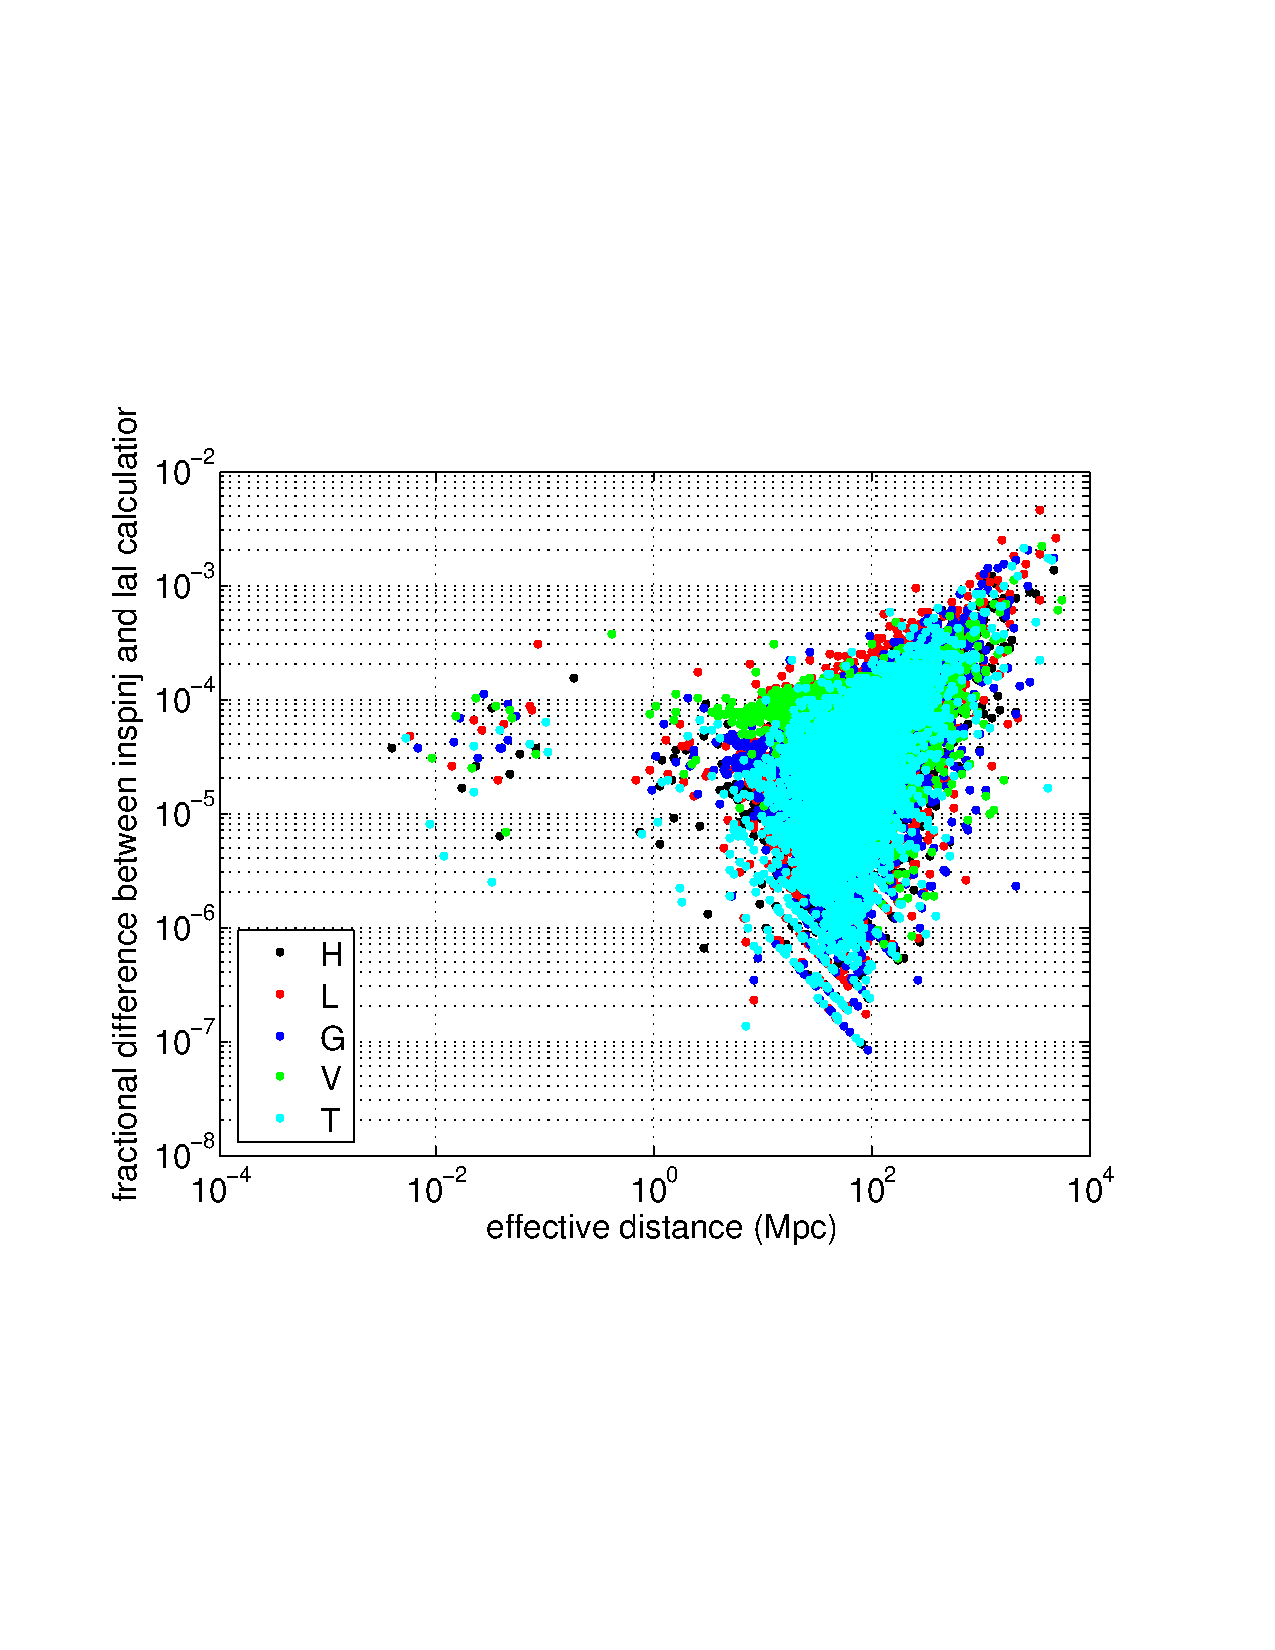
\includegraphics[width=0.9\textwidth]{figures/effective_distance_comparison}
\caption{Comparison of effective distance computed by inspinj.c and LAL
routines}
\label{fig:eff_dist_comparison}
\end{center}
\end{figure}
%
The algorithm to calculate effective distances described above is completely
contained within inspinj.c.  There is an independent method of computing
effective distances can also be called by inspinj.  It is contained in the LAL
function \texttt{LALPopulateSimInspiralSiteInfo()}.  This function populates
the site end time and effective distance for all the interferomter sites.  It
makes use of LAL functionality in the tools and date packages.  These same
functions are used when generating the injection waveform which is added to
the data stream (in lalapps\_inspiral).  As a check that these two
calculations produce the same effective distance, lalapps\_inspinj was run
twice, once with the \texttt{--lal-eff-dist} option and once without.  Figure
\ref{eff_dist_comparison} shows the fractional difference in effective
distance between the two methods for a set of injections.  We see that the
distances agree within 1\% for all injections, with the largest differences
occuring for the largest effective disances, i.e.  close to the dead spot of
the instrument.  For injections which initial LIGO is sensitive to, the
accuracy is few $\times 10^{-4}$.  

\item[Environment]\leavevmode
\begin{entry}
\item[LALAPPS\_DATA\_PATH] Directory to look for the default mass
file \verb+BNSMasses.dat+ and the default source file \verb+inspsrcs.dat+.
\end{entry}


\item[Author] 
Jolien Creighton, Patrick Brady, Duncan Brown
\end{entry}


